\chapter{Related Work}
\label{ch:state_of_the_art}

Perlin - An Image Synthesizer \cite{Perlin:1985}\\
Peachey - Modeling Waves and Surf \cite{Peachey:1986}\\
Fournier - A simple model of ocean waves \cite{Fournier:1986}\\
Mastin - Fourier Synthesis of Ocean Scenes \cite{Mastin:1987}\\
Ts'o - Modeling and rendering waves: Wave-tracing using beta-splines and reflective and refractive texture mapping \cite{Ts'o:1987}\\
Premoze - Rendering Natural Waters \cite{Premoze:2000} \\
Tessendorf - Simulating Ocean Water \cite{course:simulatingocean}

\begin{figure}
 \centering
 \subtop
 {
  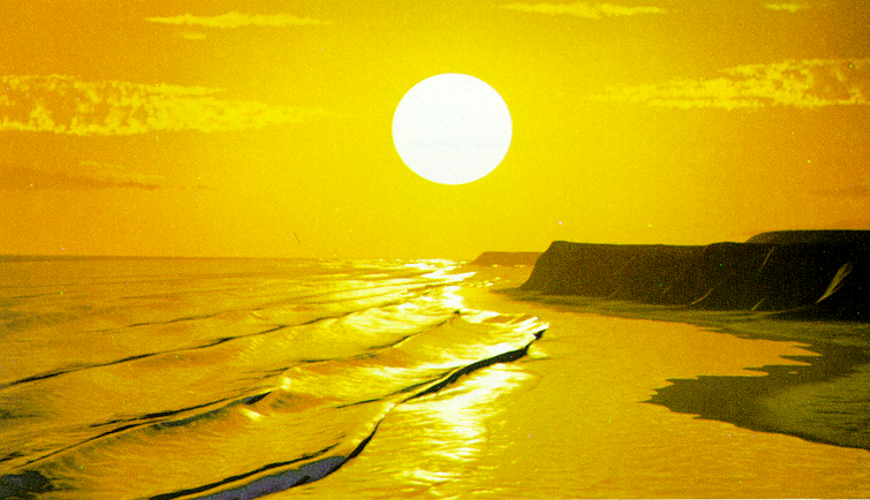
\includegraphics[scale=0.25]{figures/A_Simple_Model_of_Ocean_Waves_-_Fournier_1986-008.png}
 }
 \hfill
 \subtop
 {
  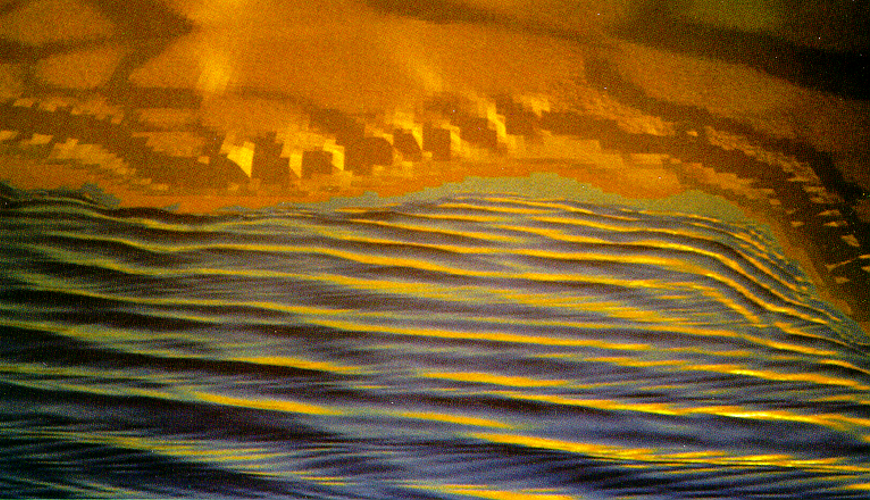
\includegraphics[scale=0.25]{figures/A_Simple_Model_of_Ocean_Waves_-_Fournier_1986-010.png}
 }
 \subtop
 {
  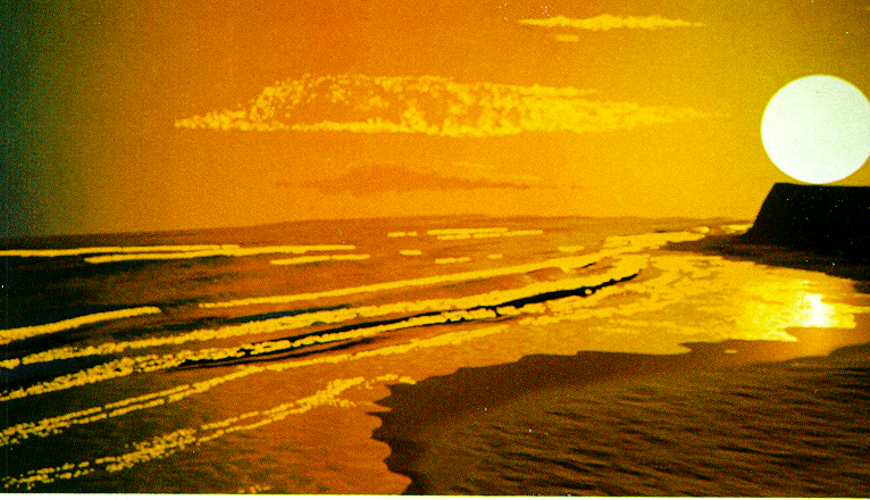
\includegraphics[scale=0.25]{figures/A_Simple_Model_of_Ocean_Waves_-_Fournier_1986-011.png}
 }
 \hfill
 \subtop
 {
  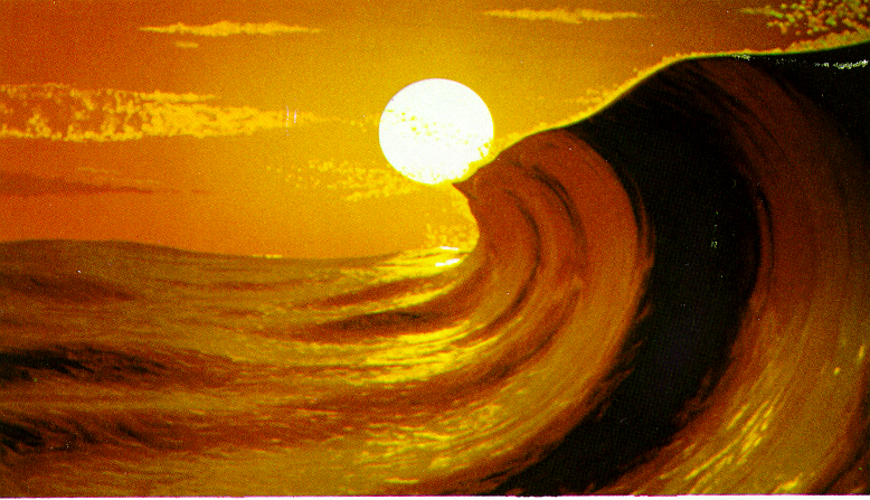
\includegraphics[scale=0.25]{figures/A_Simple_Model_of_Ocean_Waves_-_Fournier_1986-013.png}
	}
\end{figure}

\begin{figure}
 \centering
 \subtop
 {
  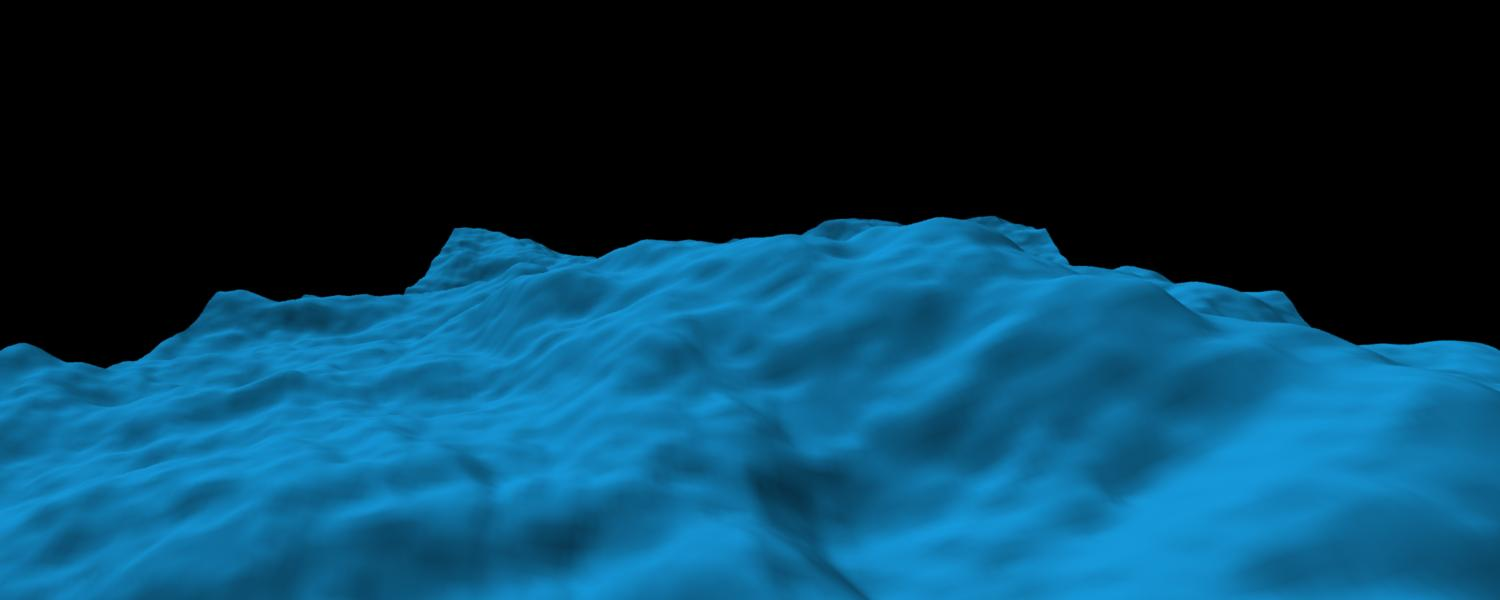
\includegraphics[scale=0.125]{figures/Simulating_Ocean_Water-012.png}
 }
 \subtop
 {
  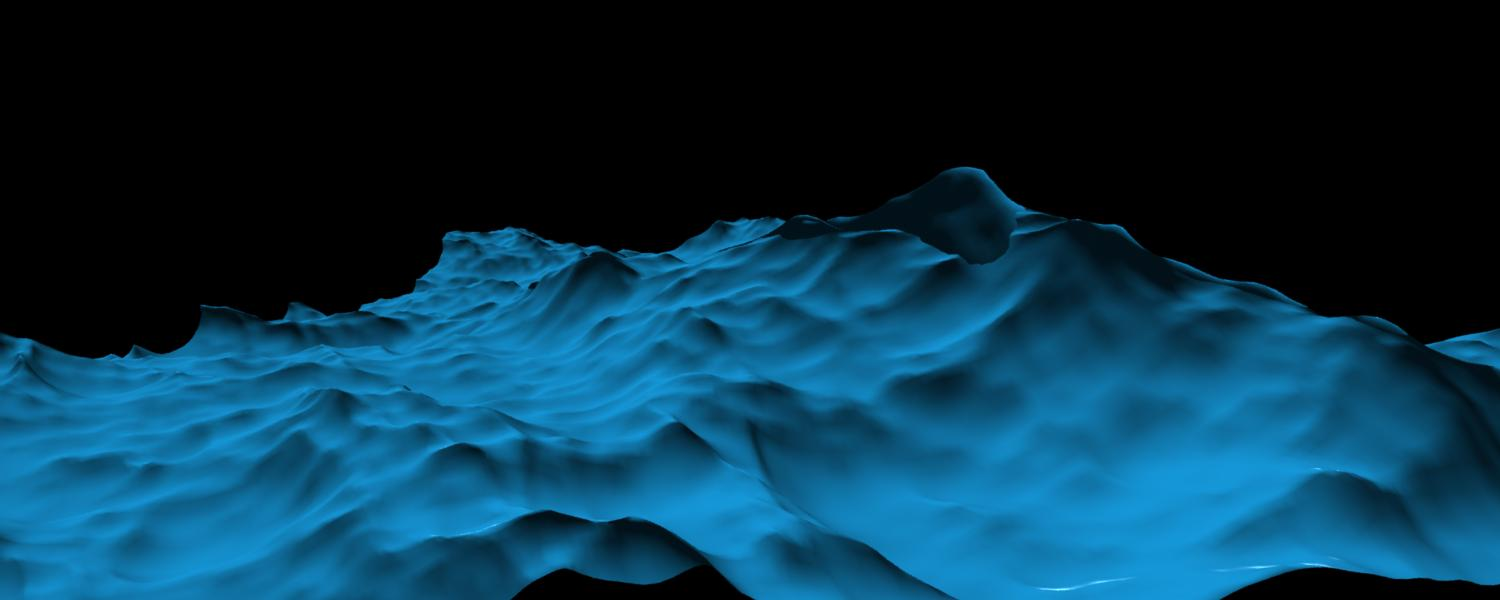
\includegraphics[scale=0.125]{figures/Simulating_Ocean_Water-013.png}
 }
\end{figure}

\begin{figure}
 \centering
 \subtop
 {
  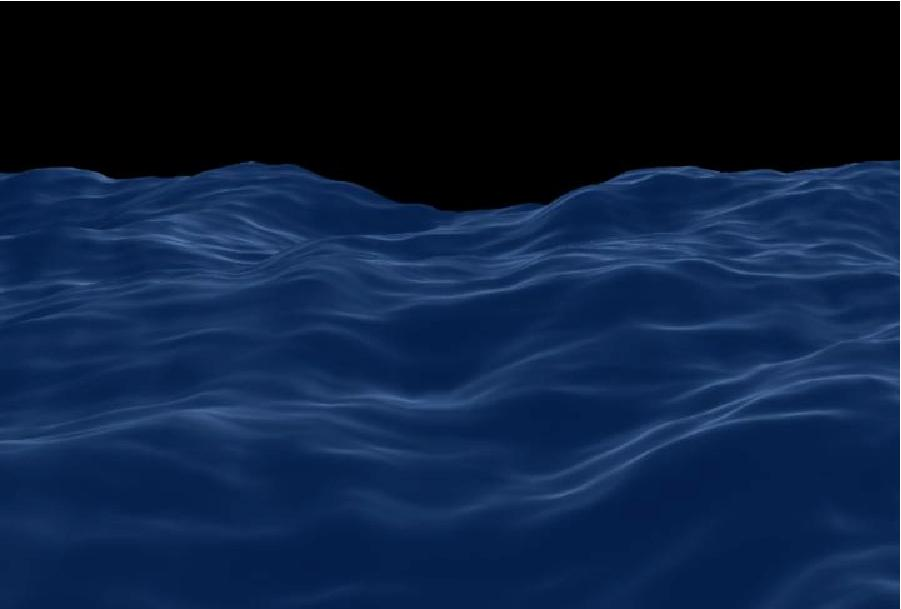
\includegraphics[scale=0.145]{figures/Simulating_Ocean_Water-008.png}
 }
 \hfill
 \subtop
 {
  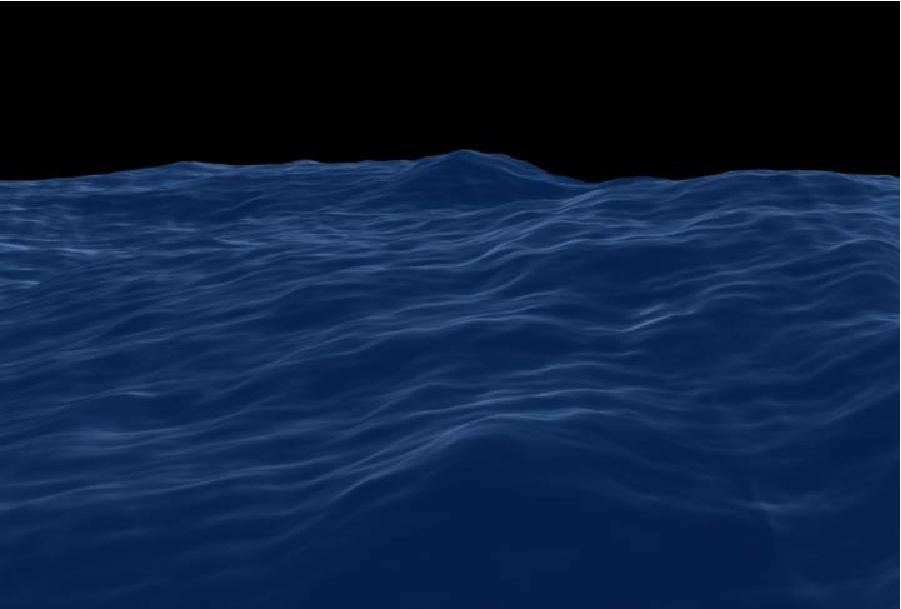
\includegraphics[scale=0.145]{figures/Simulating_Ocean_Water-009.png}
 }
 \hfill
 \subtop
 {
  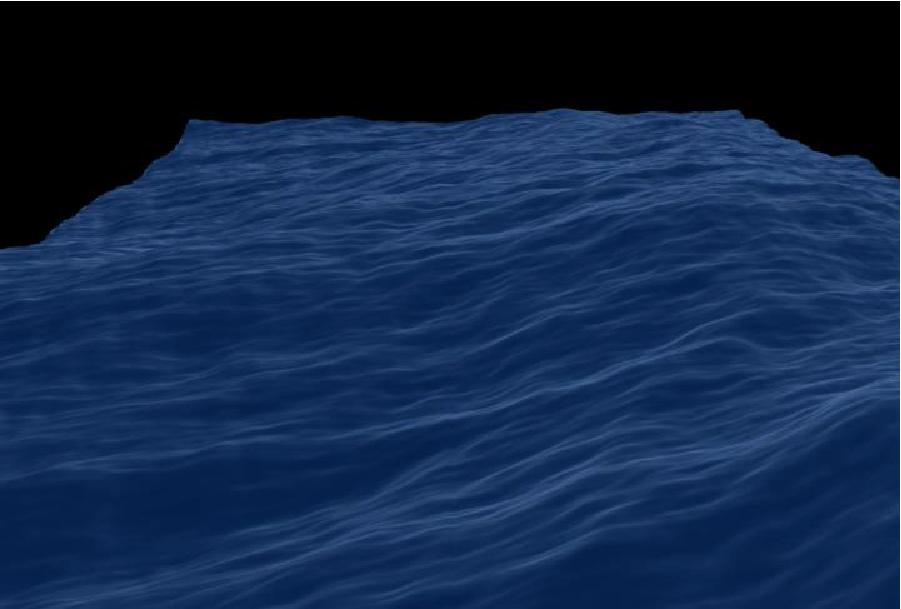
\includegraphics[scale=0.145]{figures/Simulating_Ocean_Water-010.png}
 }
\end{figure}